\documentclass[12pt]{article}

\usepackage[a4paper,left=2cm,right=2cm,top=2cm,bottom=4cm]{geometry}
\usepackage[T1]{fontenc}
\usepackage{inconsolata}
\usepackage{xcolor}
\usepackage[utf8]{inputenc}
\usepackage{ngerman}
\usepackage{amsmath}
\usepackage{amssymb}
\usepackage{listings}
\usepackage{realboxes}
\usepackage{hyperref}
\usepackage{tikz}
\usepackage{float}
\usepackage{booktabs}
\usepackage{amsmath}
\usepackage{mdframed}
\usepackage{footnote}
\usepackage{graphicx} 
\usepackage{varwidth}
\usepackage{syntax}
\newcommand\Umbruch[2][3cm]{\begin{varwidth}{#1}\centering#2\end{varwidth}}

\definecolor{pblue}{rgb}{0.13,0.13,1}
\definecolor{pgreen}{rgb}{0,0.5,0}
\definecolor{pred}{rgb}{0.9,0,0}
\definecolor{pgrey}{rgb}{0.46,0.45,0.48}
\definecolor{mygray}{rgb}{0.9,0.9,0.9}

\usepackage[hang]{footmisc}
\setlength{\footnotemargin}{-0.8em}

\lstset{language=Java,
  backgroundcolor=\color{mygray}
  showspaces=false,
  showtabs=false,
  breaklines=true,
  showstringspaces=false,
  breakatwhitespace=true,
  commentstyle=\color{pgreen},
  keywordstyle=\color{pblue},
  stringstyle=\color{pred},
  basicstyle=\ttfamily,
  moredelim=[il][\textcolor{pgrey}]{$$},
  moredelim=[is][\textcolor{pgrey}]{\%\%}{\%\%}
}

\newcommand{\type}[1]{<\negthickspace\text{#1}\negthickspace> }


\title{Code -- und Architekturanalyse}
\author{
        Klaus-Johan Ziegert\\
        MIN-Fakultät\\
        Fachbereich Informatik\\
        Studiengang: Informatik\\
        Matrikelnummer: 6523629\\
}
\date{\today}



\begin{document}
\maketitle
\begin{abstract}
        ~\\
        Diese Seminarausarbeitung dient der Vorbereitung des
        Masterprojektes ``Software-Engineering''. Das Ziel des
        Projektes ist die Entwicklung eines Werkzeuges, das die
        Analyse von bestehenden Softwaresystemen am Touchtisch
        und das Verstehen einer Software im Team ermöglicht. Um
        dieses Vorhaben zu verwirklichen, sind Kenntnisse von
        Code- und Architekturmetriken sowie der Umgang von
        existierenden Werkzeuge notwendig, die in dieser
        Ausarbeitung vorgestellt werden.  Zum Schluss werden
        Empfehlungen gegeben, welche Tools in das neue Werkzeug
        integriert werden sollten.
\end{abstract}

\newpage

\tableofcontents

\newpage

\section{Einleitung}
Diese Seminarausarbeitung dient der Vorbereitung des
Masterprojektes ``Software-Engineering''. Das Ziel des Projektes
ist die Entwicklung eines Werkzeuges, das die Analyse von
bestehenden Softwaresystemen am Touchtisch und das Verstehen
einer Software im Team ermöglicht. Um dieses Vorhaben zu
verwirklichen, sind Kenntnisse von Code- und Architekturmetriken
sowie der Umgang von existierenden Werkzeuge notwendig, die in
dieser Ausarbeitung vorgestellt werden.  Zum Schluss werden
Anreize gegeben, welche Tools in das neue Werkzeug integriert
werden sollten.

% \paragraph{Vorgehen}
% Im Kapitel \ref{metriken} wird die Definition, die Visualisierung
% als auch der allgemeine Umgang von Softwaremetriken beschrieben
% und erläutert. Daraufhin folgt im Kapitel \ref{codem} die
% Vorstellung von Codemetriken, eine detaillierte Beschreibung von
% CK-Metriken und die Untersuchung der CK-Metriken mit dem Tool
% ``geiler Tool'' an der Beispielsoftware ``verbesserungswürdige
% Software''.  Analog folgt Kapitel \ref{archm} mit den
% Archtiekturmetriken.  Als Vertreter von Archtiekturmetriken
% werden die weit bekannten Martins Metriken dienen und mit dem
% Tool ``geiler Tool'' am selbigen Beispielsoftware untersucht. Im
% vorletzten Kapitel \ref{tools} werden die unterschiedlichen Tools
% gegenübergestellt.  Der letzten Kapitel \ref{ausblick} dient als
% Ausblick für den zu entwerfenden Werkzeug, also wie und welche
% umgesetzte Metriken von den vorgestellten Tools in das neue
% Werkzeug integriert werden sollten.


\section{Softwaremetriken}\label{metriken}

Im Folgenden werden die Grundlagen der Software-Analyse mit
Softwaremetriken behandelt. Hierzu werden die Anwendungsgebiete
von Metriken beschrieben und dann spezifisch auf statische
Software-Metriken und dem Entwurf von Regeln eingegangen.
Daraufhin werden Lösungsansetze für die Bestimmung von
Schwellenwerten für den Aufbau von Regeln vorgestellt. Zum Schluss
wird ein kleiner Exkurs des Analysewerkzeug JArchitect
eingegangen, das als Voraussetzung für die nächsten Kapiteln
dienen.

\subsection{Definition von Metriken und Anwendungsgebiete}

Eine Softwarequalitätsmetrik (abk. Metrik) ist eine Funktion, die
eine Software-Einheit in einen Zahlenwert abbildet, welcher als
Erfüllungsgrad einer Qualitätseigenschaft der Software-Einheit
interpretierbar ist \cite{Wik18a}. 
Metriken können demnach abhängig von der untersuchten
Software-Einheit folgende Analysen unterstützen:
\\
\\
\textbf{Statische Analyse.} Die statistische Analyse ist ein
statisches Testverfahren, das zur Übersetzungszeit ausgeführt
wird. Der Quelltext wird als Software-Einheit herangezogen und
einer Reihe von formalen Prüfungen unterzogen, bei denen vor der
Ausführung bestimmte Sorten von Fehlern entdeckt werden \cite{Wik18b}.
Statische Metriken, die auf den ganzen oder Teile des Quelltextes
angewandt werden, können hier Aufschluss über die \textit{innere
Qualität} von Software geben. Damit sind die Qualitätskriterien
Wartbarkeit, Erweiterbarkeit, Analysierbarkeit und Testbarkeit zu
verstehen \cite[4]{Gru17}. Ein bekannter Vertreter ist die
Zeilenanzahl einer Softwarekomponente (Lines of Code, LOC).
\\
\\
\textbf{Dynamische Analyse.} Die dynamische Analyse ist ein
dynamisches Testverfahren, das zur Programmlaufzeit Fehler aufdeckt, die
in Abhängigkeit von dynamischen Laufzeitparametern auftreten; wie
variierende Eingabeparameter, Laufzeitumgebung oder
Nutzer-Interaktion \cite{Wik18c}. Im Gegensatz zu den statischen
Metriken können dynamische Metriken Aussagen über die
\textit{äußere Qualität} von Software treffen, wie z.B. der
Effizienz und der Zuverlässigkeit. Ein Vertreter ist die Anzahl
der empfangenen Nachrichten eines Objektes von anderen Objekten
(Import Object Coupling, IOC) \cite{Chh10+}.
\\
\\
\textbf{Historische Analyse.} 
Versionskontrollsysteme, wie z.B. Git oder SVN, erfassen Änderungen
des Quelltextes mit einem Zeitstempel und werden durch sogenannte Commits
festgehalten. Aus
den Commits lassen sich Vorversionen einer Software
zurückgewinnen und die historische Entwicklung sowohl von
statischen als auch dynamischen Maßzahlen verfolgen.  Aus den
Zeitdiagrammen können negative Trends der Maßzahlen vorhersagt
und zukünftig entgegengewirkt werden.
% Diese Ausarbeitung beschränkt sich im Folgenden ausschließlich
% auf die statische Analyse von objekt-orientierter Software.
% D.h. unter anderem, dass die Leistung der ausgeführten Software
% oder die Entwicklungsgeschichte nicht betrachtet wird.
% Hiermit kann bspw. beurteilt werden, wie komplex bzw.
% wartungsfreundlich ein in Java programmiertes Softwaresystem ist.
\subsection{Statische Metriken und Regeln in der OOP}

Aufgrund der hierachischen Struktur von objekt-orientierter
Software bietet es sich an, statische Metriken auf die
Hierachienebenen
Packages,
Klassen, Methoden und Felder anzuwenden.
% Da die
% Software-Architektur sich tendenziell mit Packages beschäftigt,
% werden solche hier als Architekturmetriken und die
% anderen Metriken als Codemetriken bezeichnet.\\ \\
% Eine Metrik wird nicht auf das ganze Projekt angewendet.  Hierfür
% wird die hierachische Struktur der OOP ausgenutzt, d.h. man
% wendet die Metriken auf Packages, Klassen, Methoden und Felder an.  So
% können die ermittelten Maßzahlen eines Komponententypes miteinander
% verglichen werden. 
Die Notation einer Metrik wird hier mit dem 
Namen der Metrik \textbf{metricname}, die
Komponentenebene $\type{level}$ und die Domäne $D$ wie folgt
spezifiziert:
\[
        \text{\textbf{metricname}}: ~ 
        \type{level}
        ~ \longrightarrow ~ D 
\]
% \textbf{Beispiel.} Um die Quantität einer Methode zu bestimmen,
% kann die Anzahl der Codezeilen der Methode gezählt werden. In der
% Literatur wird häufig der Name \textbf{MLOC} (Method Lines of Code)
% verwendet, sodass folgendes gilt:
% \[
%         \text{\textbf{MLOC}}: ~ 
%         \type{method}
%         ~ \longrightarrow ~ \mathbb{N} 
% \]
% Hiermit wird aufgrund des Types \type{method} klar, dass
% \textbf{MLOC} ausschließlich auf Methoden angewendet wird.
% Die Domäne $\mathbb{N}$ macht zusätzlich deutlich, dass es sich
% hier um eine Aufzählung handelt.
% \\
% \\
Neben der Klassifikation der Metriken durch ihre Ebene und Domäne
werden in \cite{Sne10} folgende Unterteilung vorgeschlagen:
\\
\\
\textbf{Quantitätsmetrik.} Quantitätsmetriken liefern den Umfang
einer Komponente. Die Domäne ist meistens auf die natürliche
Zahlen $\mathbb{N} \cup 0$ festgelegt oder durch eine bekannte
obere Grenze auf $[0,1] \subset \mathbb{R}$ normiert. Eine hohe
Maßzahl solcher Metriken weisen auf eine entsprechend hohe
Systemintelligenz hin. Einer Vertreter dieser Metrikart ist das
schon vorgestellte LOC. Für Methoden wird die Metrik MLOC 
daher bspw. wie folgt spezifiziert:
\[
        \text{MLOC}: ~ 
        \type{method}
        ~ \longrightarrow ~ \mathbb{N}
\]
\textbf{Komplexitätsmetrik.} Komplexitätsmetriken messen die
Beziehungen zwischen den Komponenten. Die Domäne gleicht der 
Domäne von Quantitätsmetriken. Assoziationen wie Vererbung sind
in der OOP ausgelegt, sollten jedoch für das Verständnis des
Softwaresystem
nicht ausarten. Ein Vertreter dieser Metrikart ist z.B. die Anzahl der
Kinder einer Klasse in der Vererbungshierachie (NOC, Number of
Children) (vgl. Kap. \ref{sec:NOC}):
\[
        \text{NOC}: ~ 
        \type{class}
        ~ \longrightarrow ~ \mathbb{N} \cup \left\{ 0
        \right\}
\]
\textbf{Qualitätsmetrik.} Qualitätsmetriken geben die Erfüllung
oder den Erfüllungsgrad von Regeln wieder. Die Domäne ist auf
$[0,1] \subset \mathbb{R}$ oder binär $\mathbb{B}$ festgelegt.
Binäre Qualitätsmetriken, auch einfach Regel genannt, können
durch Filtern und Kompositionen anderer Metriken konstruiert
werden. Dabei weisen Regeln lediglich  mit
hoher Wahrscheinlichkeit auf einen Designfehler hin. Ein Vertreter dieser Metrikart
ist die Regel der Gottesklasse (GodClass) (vgl. Kap.
\ref{sec:Identifikation von Gottklassen}):
\[
        \text{GodClass}: ~ 
        \type{class}
        ~ \longrightarrow ~ \mathbb{B} 
\]
Für Entwickler von Softwaresystemen sind Regeln für das schnelle
Erkennen von Komponenten hilfreich, deren Maßzahlen mit
erhöhter Wahrscheinlichkeit auf einen Designfehlern hinweisen.
In \cite{Mar04} wird für die Konstruktion von Regeln die
sogenannte \textit{Detection Strategie} vorgeschlagen, dass nach
dem Filter- und Kompositionsprinzip funktioniert. Abweichungen
von guten Designprinzipien und Heuristiken, wie z.B. die genannten Gottklassen,
werden durch Metriken mit festgelegten Schwellenwerten und
Kompositionsoperatoren \textsf{and}, \textsf{or} und
\textsf{butnot} zu quantifizierbaren Ausdrucke zusammengefasst.
% In der Backus-Naur-Form unterliegen solche Ausdrucke der
% folgenden Syntax \footnotemark:
% \begin{grammar}
% <exp> ::= <com>
%
% <com> ::= <com> \textsf{and} <com> | <com> \textsf{or} <com>
% | \textsf{butno} <com> | <filt>
%
% <filt> ::= <metric> \textsf{less than} <value> | <metric>
% \textsf{greater than}
% <value>
%
% <metric> ::= LOC | NOC | \dots (''alle Metriken einer
% Komponente'')
%
% <value> ::= (''reele Werte'')
% \end{grammar}
% %
% \footnotetext{Die syntaktische Form ist ein Binärbaum.
% Klammerersparnisregeln und
% synaktischer Zucker lassen sich in die Form für die Vereinfacherung der
% Schreibweise einfließen.}
% %
\\
\\
Die Auswertung eines quantifizierbaren Ausdruck ist in Abb.
\ref{fig:filter} dargestellt. Aus Metriken und zugehörigen
Schwellenwerten werden aus den untersuchenden Komponentenmengen
$\left( M_{n} \right)_{n \in \mathbb{N}}$ die Ergebnismengen
$\left( F_{n}\right)_{n \in \mathbb{N}}$ gefiltert. Anschließend
evaluiert man die Kompositionsoperationen entsprechend ihrer
mengenorientierter Semantik. Dies erfolgt solange bis die
endgültige Ergebnismenge bestimmt wird. Die Komponente in der
endgültigen Ergebnismenge verstoßen dann mit erhöhter
Wahrscheinlichkeit gegen einen spezifisches Designprinzip oder
einer Heuristik.  Solche Komponenten müssen dann von den
Entwicklern genauer untersucht und anschließend abgewägt werden,
ob die Aussage von Designfehlern seine Richtigkeit hat.
\begin{figure} 
  \centering
  \makebox[\textwidth][c]{\includegraphics[width=.6\textwidth]{../Images/filter.png}}
  \caption{Das Filter- und Kompositionsprinzip aus der
          mengenorientierten Sicht \cite{Mar04}}
  \label{fig:filter}
\end{figure}
% Unter
% Qualitätsmetriken versteht man Indikatoren von Bad Smells, wie
% z.B. Redundanz von Code, zu lange Methoden (''Brain-Methods''),
% Gottklassen usw.

\subsection{Bestimmen von Schwellenwerten}

Wenn die Maßzahl einer Komponente ermittelt wird, dann stellt
sich die Frage, ob dieser Wert nicht der Norm entspricht oder
eine weite Distanz zu gewünschten Maßzahlen aufweist. Die
Entscheidung von abnormalen Werten wird dabei -- wie in der
\textit{Detection Strategie} behandelt -- durch Schwellenwerte
getroffen.  Dabei gibt es keine universelle Schwellenwerte, da
etliche Faktoren, wie die gewählte Programmiersprache, der
Anwendungskontext, die Konvention usw., dies nicht zulassen.  Es
ist daher essentiell eigene Schwellenwerte zu ermitteln oder den
Hintergrund von empfohlenen Schwellenwerte zu verstehen und
abzuwägen, ob der Untersuchungskontext dieser ermittelten Werte
zum eigenen Softwaresystem passt.  In \cite{Lan07} werden zwei
Strategien zur Bestimmung von Schwellenwerten präsentiert: 
\\
\\
\textbf{Statistische Schwellenwerte}. Liegt die Domäne der zu
untersuchenden Metrik bei den natürlichen Zahlen $\mathbb{N}$,
bieten sich statistische Schwellenwerte an.  Man wählt eine Menge
von Softwaresystemen, die zum untersuchenden Softwaresystem
ähnlich sind, und berechnet für jede Metrik den
Durchschnitt AVG und die Standardabweichung STDEV. Hiermit können
die Schwellenwerte Lower margin, Higher margin und Very high, wie
in der Abb. \ref{fig:statistisch} dargestellt, abgeschätzt
werden.
		\begin{figure}
                        \centering
		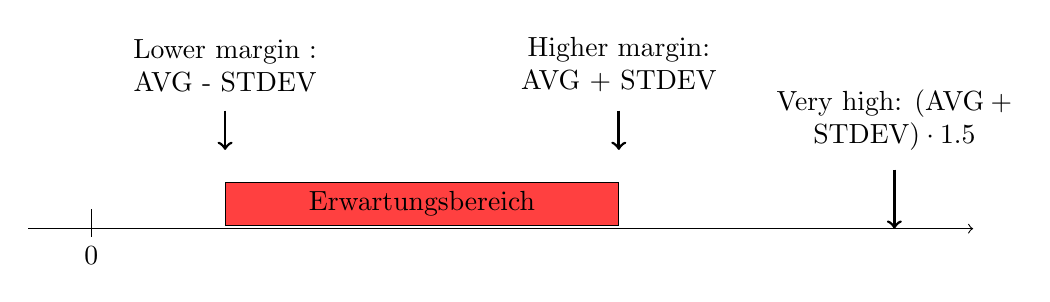
\begin{tikzpicture}
			\draw[->] (0,0) -- (12,0);
			\foreach \x in {0.8}
			\draw(\x cm,7pt) -- (\x cm, -3pt);
			\draw (0.8,0) node[below=3pt] {$0$};
			\draw (5,0)
			node[rectangle,above=1pt,draw=black,fill=red!
				75,
			minimum width=5cm]
			{Erwartungsbereich};
			\draw[->, line width=1pt] (2.5,1.5)
			node[above=3pt]
                        {\Umbruch{Lower margin : AVG - STDEV}}-- (2.5,1) ;
			\draw[->, line width=1pt] (7.5,1.5)
			node[above=3pt]
                        {\Umbruch{Higher margin: AVG + STDEV}}--
			(7.5,1) ;
			\draw[->, line width=1pt] (11,.75)
			node[above=3pt]
                        {\Umbruch{Very high: $(\text{AVG} +
                        \text{STDEV}) \cdot 1.5$}}--
			(11,0) ;
		\end{tikzpicture}
		\caption{Statistische Schwellenwertempfehlung aus
                        \cite{Lan07}}
                        \label{fig:statistisch}
	\end{figure}
Dabei ist Vorsicht geboten, da Ausreißer, die nicht in die
erwartete Messreihe passen, die gewünschten Grenzen verzerren.
Solche Ausreißer müssen daher durch Ausreißertests vorher
entfernt werden.  Eine Ausnahme besteht jedoch, wenn man
stattdessen die Messreihe auf das eigene Softwaresystem
beschränkt und systemspezifische Anomalien auf untere
Hierarchieebene, abwärts der Klassenebene, auffinden möchte.  Auf
der Packageebene ist nämlich die Anzahl der Messreihe häufig
nicht erwartungsgetreu.
Wohingegen eine zu untersuchende Maßzahl
außerhalb des Bereiches von Lower und Higher margin schon ein von
der Norm abweichender Wert zu zusprechen ist, können Komponente
mit Maßzahlen die sogar außerhalb von Very High hinausgehen, als
Anomalien identifiziert werden. 
\\
\\
\textbf{Sinnvolle Schwellenwerte (engl. Meainingful Thresholds)}.
Ist die Domäne auf $D = [0,1] \subset \mathbb{R}$ normiert, so
sind aus der Statistik folgende Grenzen wohlbekannt:
\begin{itemize}
        \item 0.25 - One Quarter
        \item 0.33 - One Third 
        \item 0.5 - Half
        \item 0.66 - Two Thirds 
        \item 0.75 - Three Quarters 
\end{itemize}
Im Gegensatz zu den statistischen Schwellenwerte sind aus dem
Verständnis der Metriken eine oder mehrere gewünschte Maßzahlen
anzustreben.  Es ist z.B. das Ziel bei den Martin-Metriken
Instabilität I und Abstrakion A einen Ausgleich der Maßzahl
anzustreben, also einen Wert bei Half (vgl.  Kap. \ref{I} und
\ref{A}).  Daher bietet es sich für solche Metriken an,
Schwellenwerte bei One Quarter und Three Quarters für die
feingranulare Analyse und die Schwellenwerte One Third und Three
Quarters für die grobgranulare Analyse auszuwählen.
\\
\\
Ebenso können absolute Werte in sinnvolle Schwellenwerte
unterteilt werden. Das menschliche Kurzzeitgedächtnis hat eine
Gedächtnisspanne von etwa 7-8 Elemente \cite{Mil56}. Aus dieser
Kenntnis können folgende Schwellenwerte angegeben werden:
\begin{itemize}
        \item 0 - None
        \item 1 - One/Shallow
        \item 2--5 - Two, Three/Few/Several
        \item 7--8 - Short Memory Capacity
\end{itemize}
Für Entwickler ist es nämlich günstig Komponente im Überblick zu
haben. Bspw. kann der Umgang von globalen Variabeln einer Klasse
mit mehr als der Short Memory Capacity hierdurch als fraglich
bestimmt werden.

\subsection{Analysewerkezeug JArchitect}

Das Analysewerkzeug JArchitect ist ein statistisches Werkzeug für
Java-Code \cite{Get18}. Das Tool bietet eine Vielzahl von Metriken
und Regeln an, die dann für Analysezwecken mit unterschiedlichen
Darstellungen visualisiert werden kann. Zudem können eigene
Regeln mit der Abfrage-Sprache CQLINQ erstellt und in das System
von JArchitect integriert werden. Im Folgenden wird ein kleiner
Exkurs zum Schreiben einer einfachen Regeln und entsprechender
Visualisierung mit einem Tree Map für das Projekt Sweet Home 3D
präsentiert.
\\
\\
\textbf{Definieren von Regeln mit CQLinQ.} JArchitect umfasst 82
Metriken und eine Vielzahl von empfohlenen Regeln. Nach der
Analyse eines Projektes mit JArchitect sind die Maßzahlen der
Metriken berechnet und die Regeln evaluiert, dessen potenzielle
Regelverstöße in einem Dashboard zusammengefasst werden. Um
empfohlene Regeln dem Projekt anzupassen oder eigene Regeln zu
schreiben, kann man den CQLinQ-Editor nutzen. CQLinQ (Code Query
Linq) ist ein ähnliches Abfragesystem wie SQL mit dem
Unterschied, dass Sprachelemente zur Verfügung stehen, die den
Zugriff von hierachischen Strukturen der OOP angepasst ist. Für
jeden Komponententypen sind die Maßzahlen als Metrikattribute in
einer Tabelle gespeichert und können deskriptiv abgefragt werden.
\\
\\
Als Beispiel soll die Anfrage als einfache Regel im oberen
Teilfenster und die Ausgabe im unteren Teilfenster in der Abb.
\ref{fig:Bild4} dienen. Das Ziel dieser Regel ist, Packete zu
ermitteln, die mehr als 6000 Codezeilen haben. Hierzu wird die
Tabelle JustMyCode.Packages angesprochen.  JustMyCode ist
essentiell, da ansonsten auch sogenannte ThirdParty Packages
mitberücksichtigt werden; das sind importierte Packages außerhalb
des Projektes.  Mit der Anweisung „Where“ wird die Bedingung
spezifiert, dass NBLinesOfCode (LOC) zum Erfüllen der Regel
größer als 6000 sein soll.  In der nächsten Zeile wird die
Ausgabe definiert, dabei soll der Projektname als auch die
Codezeilen zurückgegeben werden. Im unteren Teilfenster ergibt
die Anfrage zwei Packages, nämlich com.eteks.sweethome3d.swing
mit 15.886 Codezeilen und com.eteks.sweethome3d.viewcontroller
mit 9.806.  Wenn 6000 Codezeilen ein Kriterium für einen
schlechten Design gewünscht wird, dann kann vor der Anfrage die
Anweisung „warnif > 0“ angehängt und gespeichert werden. Bei der
nächsten Analyseauswertung, wird die Anfrage in das
Warnungssystem berücksichtig und eine diesbezügliche Warnung
wegen diesen beiden Packages ausgegeben.
\begin{figure} 
  \centering
  \includegraphics[width=0.7\textwidth]{../Images/SchwellenwertLineofCode.PNG}
 \caption{Drittes Bild}
  \label{fig:Bild3}
\end{figure}
~\\ 
\\
\textbf{Visualisieren mit Tree Map.} Das Analysewerkzeug
JArchitect bietet u.a. ein Tree Map für die Visualisierung von
Maßzahlen, das die hierachische Struktur der OOP unterstützt.
Für jede Komponente wird ein Rechteck erstellt und die Rechtecke
werden abhängig von ihrer Enthält-Beziehung miteinander
verschachelt. Das ganze Projekt als Rechteck enthält Rechtecke
als Packages, Packages enthalten Klassen und Klassen enthalten
Methoden oder Felder. Mit der Option \textit{Level} lässt sich
ein Komponententyp auswählen; damit werden die in der Hierachie
darunterliegenden Komponententypen nicht mehr angezeigt. Neben
dieser Option bietet JArchitect zwei weitere nützliche Optionen an:
\begin{itemize}
        \item \textit{Code Metric} bestimmt die proportionale 
                Rechteckgröße des ausgewählten
                Komponententyps mit der Auswahl einer Metrik.
        \item  Durch das Aktivieren von \textit{Color}
               kann eine weitere Metrik ausgewählt werden, dass  
               die Rechtecke abhängig von der Maßzahl farbig
               gestaltet.
\end{itemize}
Zur Demonstration wird weiterhin das Projekt Sweet Home 3D
herangezogen. In der Abb. \ref{fig:Bild1} ist das zugehörige
Treemmap dargestellt. Hierzu ist als \textit{Level} der
Komponententyp Package, als \textit{Code Metric} (in der
Darstellung als Size angegeben) mit der Metrik LOC gesetzt und
\textit{Color} ebenfalls mit der Metrik LOC aktiviert. Durch das
Gleichsetzen der Metriken von \textit{Color} und \textit{Code
Metric} korrespondieren beide Attribute miteinander; ein großer
Rechteck kann nur rot und ein kleiner Rechteck kann nur grün
sein. Aus dieser Darstellung erkennt man klar, dass es sich um 11
Projekte handelt, wohingegen das Package com.eteks.sweethome3d
überproportional viele Codezeilen hat.  Die zwei größten Packages
ergeben zusammen mehr als die Hälte der Codezeilen, dass die
These aufstellen lässt, dass die Systemintelligenz ungünstig
verteilt ist.
\\
\\
In der Abb. \ref{fig:Bild2} ist das gleiche Tree Map nur mit den
Unterschied, dass das \textit{Level} auf Method gesetzt ist.
Vergleicht man dies mit der Abb. \ref{fig:Bild1}, so sind die
Projekt-Rechtecke noch einigermaßen erkennbar. Die Rechtecke,
dessen Ecken dunkel schraffiert sind und selber kleine Rechtecke
enthalten, stellen hier Klassen dar. Die elementare Rechtecken
sind demzufolge die Methoden. Die Methoden, die rot eingezeichnet
sind, haben etwa 200 Zeilen Code. Dies lässt sich nämlich im
Farbspektrum am rechten Rand des Fensters feststellen.  Die
Codezeilen scheinen in der Methodenebene ungefähr gleichmäßig
verteilt sein, da relativ wenige Methoden die Farbe rot
aufweisen.
\\
\\
Anstelle einer Metrik wie LOC kann ebenfalls das Ergebnis einer
Regel auf einen Tree Map angewandt werden. In Bezug auf der
einfachen Package-Regel in der Abb. \ref{fig:Bild4} kann das Tree
Map in der Abb.  \ref{fig:Bild3} durch das Setzen der Regel als
\textit{Code Metric} gewonnen werden. Erfüllt ein Package eine
Regel, dann werden die entsprechenden Rechtecke bläulich gefärbt,
ansonsten schwarz gefärbt. In der Darstellung erkennt man dann
klar, dass die zwei bläulich gefärbten Projekte mehr als 6000
Codezeilen haben.
\begin{figure} 
  \centering
  \makebox[\textwidth][c]{\includegraphics[width=1.2\textwidth]{../Images/Visualisierung1}}
  \caption{Erstes Bild}
  \label{fig:Bild1}
\end{figure}
%
\begin{figure} 
  \centering
  \makebox[\textwidth][c]{\includegraphics[width=1.2\textwidth]{../Images/Visualisierung2}}
  \caption{Zweites Bild}
  \label{fig:Bild2}
\end{figure}
%
%
\begin{figure} 
  \centering
  \makebox[\textwidth][c]{\includegraphics[width=1\textwidth]{../Images/VisualisierungSchwellenwertLineofCode.PNG}}
  \caption{viertes Bild}
  \label{fig:Bild4}
\end{figure}



% \begin{figure}[Htbp] 
%   \centering
%      \includegraphics[width=0.7\textwidth]{bild.jpg}
%   \caption{Erstes Bild}
%   \label{fig:Bild1}
% \end{figure}
%
% \begin{figure}[Htbp] 
%   \centering
%      \includegraphics[width=0.7\textwidth]{bild.jpg}
%   \caption{Erstes Bild}
%   \label{fig:Bild1}
% \end{figure}
%
% \begin{figure}[Htbp] 
%   \centering
%      \includegraphics[width=0.7\textwidth]{bild.jpg}
%   \caption{Erstes Bild}
%   \label{fig:Bild1}
% \end{figure}


\section{Codemetriken}\label{codem}

Unter Codemetriken sind die Metriken zu verstehen, die eher die
unteren Hierachieebenen untersuchen und damit zu feingranularen
Verbesserungen der Software bewegen. Im Gegensatz zu \cite{Sne10}
werden Klassenmetriken hier ebenfalls zu Codemetriken mitgezählt.
Im Folgenden werden die sogenannten CK-Metriken eingeführt, die
leicht abgeändert u.a. für die Gottklassenregel verwendet wird
\cite{Mar04}. Darauf aufbauend wird die von \cite{Mar04}
präsentierte Gottklassenregel eingeführt und die Umsetzung in
JArchitect erläutert. 

\subsection{CK-Metriken}
\label{sec:CK-Metriken}
Der Student Chidamber und der Professor Kemerer führten sechs
Metriken für die Analyse von objekt-orientierte Software ein
\cite{chi94}. Diese Metriken haben den großen Vorteil, dass sie
relativ unabhängig sind und daher für die Entwicklung von Regeln
nützlich sind: 
~\\
\\
\textbf{WMC.} Die erste CK-Metrik ist die Anzahl gewichteter Methoden
(engl. Weighted Method Count, abk. WMC). Diese Kenngröße
misst die Summe der Komplexitäten aller Methoden einer Klasse.
In \cite{chi94} wird die Bestimmung der Komplexität einer Methode
nicht festgelegt, so kann für die Komplexität einer Methode die
Anzahl der Codezeilen (LOC) oder die häufig mit WMC vorgestellte
Zyklomatische Komplexität nach McCabe (McCabe-Metrik) verwendet werden.
\[
        \text{WMC}: ~ 
        \type{class}
        ~ \longrightarrow ~ \mathbb{N}  \cup \left\{ 0 \right\} 
\]
Diese Metrik wird häufig als ein Maß für den Entwicklung- und
Erwartungsaufwand einer Klasse verstanden. Je mehr Methoden
vorhanden oder je komplexer die Methoden sind, desto
applikationsspezifischer sind die Methoden i.d.R. und führen
daher zu einer schlechten Wiederverwendbarkeit. Eine Maßzahl über
34 ist eine statistisch ungünstige Größe (vgl.
Tab. \ref{tab:wmcthreshold}).
\begin{figure}[H]
\centering
 \begin{tabular}{lcr}
    \toprule
    Good/Common & Regular/Casual & Bad/Uncommon \\
    \midrule
    $m \leq 11$ & $11 < m \leq 34$ & $m > 34$ \\
    \bottomrule
  \end{tabular}
  \caption{Schwellenwerte für WMC aus \cite{Fil15}}
  \label{tab:wmcthreshold}
\end{figure}
~
\\~
\textbf{DIT.} Die zweite CK-Metrik ist die Tiefe der
Vererbungshierarchie (engl. Depth of Inheritance, abk. DIH).
Diese Kenngröße misst die Länge des maximalen Weges von der
Wurzel bis zur betrachteten Klasse im Vererbungsbaum. Der
maximale Weg ist dann nur von Interesse, wenn Mehrfachvererbungen
möglich sind, wie in C++
\[
        \text{DIT}: \type{class} 
        \longrightarrow \mathbb{N} \cup \left\{ 0 \right\} 
\]
Diese Metrik wird häufig als Maß für die Testbarkeit und
Codeverständlichkeit verstanden.  Je Tiefer die
Vererbungshierachie, desto mehr Methoden werden üblicherweise von
anderen Klassen geerbt. Dies führt häufig zu einem
unvorhersehbaren Verhalten einer Klasse. Eine Maßzahl von weniger
als 4 wird statistisch vorgeschlagen \ref{tab:ditthreshold}.
\begin{figure}[H]
\centering
 \begin{tabular}{lcr}
    \toprule
    Good/Common & Regular/Casual & Bad/Uncommon \\
    \midrule
    $m \leq 2$ & $2 < m \leq 4$ & $m > 4$ \\
    \bottomrule
  \end{tabular}
  \caption{Schwellenwerte für DIT aus \cite{Fil15}}
  \label{tab:ditthreshold}
\end{figure}
~\\
\\
\textbf{NOC.} Eine Ergänzung zu DIH ist die dritte CK-Metrik: die
Anzahl der Kinder in der Vererbungshierarchie (engl. Number of
Children, abk.  NOC). Diese Kenngröße gibt für eine Klasse die
Anzahl der unmittelbaren abgeleitenden Klassen (auch
Basisklassen) wieder.
\[
        \text{NOC}: \type{class} 
        \longrightarrow \mathbb{N} \cup \left\{ 0 \right\} 
\]\label{sec:NOC}
~\\
Ein hoher Wert von NOC bedeutet ein hohes Maß an
Wiederverwendung.  Je größer die Anzahl der Subklassen ist, desto
wahrscheinlicher liegt ein zu generell abstrahierte Oberklasse
vor. Es wird ein stastischer Wert von nicht größer als 3
vorgeschlagen \ref{tab:nocthreshold}.
\begin{figure}[H]
\centering
 \begin{tabular}{lcr}
    \toprule
    Good/Common & Regular/Casual & Bad/Uncommon \\
    \midrule
    $m \leq 1$ & $1 < m \leq 3$ & $m > 3$ \\
    \bottomrule
  \end{tabular}
  \caption{Schwellenwerte für NOC aus \cite{Fil15}}
  \label{tab:nocthreshold}
\end{figure}
~\\
\\
\textbf{CBO.} Die vierte Metrik einer Klasse ist die Anzahl der
gekoppelten Klassen (engl. Coupling between Object Classes, abk. CBO).
Eine Klasse A ist mit einer anderen Klasse B genau dann
gekoppelt, wenn A über eine Referenz Zugriff auf B oder umgekehrt
hat.
\[
        \text{CBO}: \type{class}
        \longrightarrow \mathbb{N} \cup \left\{ 0 \right\} 
\]
Eine exzessive Kopplung, verbunden mit einer hohen Maßzahl von
CBO, widerspricht dem modularen Aufbauansatz.  Die externe
Wiederverwendbarkeit wird aufgrund starker Abhängigkeit
erschwert.
\\
\\
\textbf{RFC.} Die fünfte CK-Metrik ist die Anzahl potenzieller
Zielmethoden (engl. Response for Class, abk. RFC). Diese
Kenngröße misst die Anzahl aller ausführbaren Methoden einer
Klasse. Zu den definierten Methoden der Klasse werden ebenfalls
die von der Instanz anderer Klassen aufgerufenen Methoden
innerhalb der Klasse mitgezählt.
\[
        \text{RFC}: \type{class}
        \longrightarrow \mathbb{N} \cup \left\{ 0 \right\} 
\]
RFC gibt eine untere Schranke für die Anzahl der Testfälle an, die
durch die möglichen Methodenaufrufen notwendig werden.
\\
\\
\textbf{LCOM.} Die letzte hier vorgestellte CK-Metrik ist der
Zusammenhalt der Methoden (engl. Lack of cohesion in methods,
abk. LCOM).  Diese Kenngröße misst die Anzahl aller möglichen
Methodenpaare, die keine Instanzvariable gemeinsam haben,
subtrahiert mit der Anzahl aller Methodenpaare, die mindestens
eine Instanzvariable gemeinsam haben. Falls die Berechnung 
zu einem negativen Ergebnis führt, wird dannf für LCOM die
Maßzahlzahl 0 angenommen. 
\[
        \text{LCOM}: \type{class}
        \longrightarrow \mathbb{N} \cup \left\{ 0 \right\} 
\]
LCOM gibt die Kohäsion der Methoden an und signalisiert bei hoher
Kohäsion eine gute Klasseneinteilung. Ein niedrige Kohäsion wird
häufig zum Anlass gegeben, eine Klassenaufteilung anzustreben.
Wird dieser Wert normiert, werden nicht höhere Wert als $0.725$
empfohlen \ref{tab:lcomthreshold}.

\begin{figure}[H]
\centering
 \begin{tabular}{lcr}
    \toprule
    Good/Common & Regular/Casual & Bad/Uncommon \\
    \midrule
    $m \leq 0.167$ & $0.167 < m \leq 0.725$ & $m > 0.725$ \\
    \bottomrule
  \end{tabular}
  \caption{Schwellenwerte für LCOM aus \cite{Fil15}}
  \label{tab:lcomthreshold}
\end{figure}
%
\subsection{Identifikation von Gottklassen}
\label{sec:Identifikation von Gottklassen}

In \cite{Mar04} wird die \textit{Detection Strategie} zum
Auffinden von Gottklassen empfohlen. Dabei werden zunächst
die Heuristiken herangezogen, die eine Gottklasse nicht einhält.
Diese lauten wie folgt:
\begin{enumerate}
        \item Top-level classes in a design should share work
                uniformly.
        \item Beware of classes with much non-communicative
                behavior.
        \item Beware of classes that access directly data from
                other classes.
\end{enumerate}
Für jede dieser Heuristiken wird anschließend eine Metrik
ausgesucht, die die entsprechende Heuristik am Besten
quantifiziert. Die erste Heuristik kann durch WMC, die zweite
Heuristik durch LCOM und die dritte Heuristik durch CBO ermittelt
werden. Für CBO hat man jedoch das Problem, dass lediglich der
einseitige Zugriff auf Instanzvariabeln, direkt oder durch
sondiernde Methoden, von Interesse ist. Deshalb wird in
\cite{Mar04} die Metrik ATFD (Access to Foreign Data) hierfür
herangezogen. Eine leicht geänderte Form wird für die zweite
Heuristik benutzt und zwar TCC (Tight Class Cohäsion), der
lediglich das Verhältnis aller direkt verbundenen Methoden zu
allen potenziellen Methoden bemisst. 
\\
\\
Nach \cite{Mar04} hängen die Schwellenwerte abhängig vom Projekt
ab. So wird für WMC die Klassen gefiltert, die in den oberen 25
\% liegen, und für TCC, die in den unteren 25 \% liegen.
Lediglich für ATFD wird der Schwellenwert auf 1 gesetzt,d.h. es
werden alle Klassen gefiltert, die einen Zugriff auf eine andere
Klasse haben.
\\
\\
Für die Kompostion werden zwei mögliche Lösungsansätze geliefert.
Der erste Lösungsansatz kann als eine grobgranulare Untersuchung
betrachtet werden, denn es werden die Filter mit \textsf{and}
vebunden. D.h. wenn eine Klasse alle drei Heuristiken verstößt,
liegt mit hoher Wahrscheinlichkeit eine Gottklasse vor.  In der
feingranulare Untersuchung wird im Gegensatz die erste Heuristik
gefordert, jedoch muss die 2. oder 3. Heuristik hierfür erfüllt
werden.

\section{Architekturmetriken}\label{archm}

Architekturmetriken sind Metriken, die auf eine höheren
Hierachieebene angewandt werden und demnach eine grobgranulare
Veränderung der Software anregt. Solche Änderungen sind dabei mit
einem großen Aufwand verbunden und sollten demnach schon im
Architekturentwurf der Software berücksichtigt werden.  Im
Folgenden werden die bekannten und Martins Metriken vorgestellt.
Anschließend erfolgt eine Analyse dieser Martins Metriken mit dem
Projekt Sweet Home 3D.

\subsection{Martins Metriken}
Im Gegensatz zu den CA-Metriken sind die Martins Metriken nicht
unabhängig und verfolgen das Ziel die sogenannte Martin-Metrik zu
berechnen. Dieser dient dann als Qualitätsmetrik, der als ein
Erfüllungsgrad einer Regel dient.
~\\
\\
\textbf{CA}.\label{CA} Die erste Martin-Metrik ist die afferente Kopplung (eng. afferent
Coupling, abk. CA).
Diese Kenngröße misst für ein Package $P$ die Anzahl der Packages,
die von Klassen innerhalb von $P$ abhängen. Man spricht daher von
der Anzahl der eingehenden Abhängigkeiten.
% Die eingehenden Abhängigkeiten werden in einem Java-Quelltext mit
% der Anweisung \lstinline|import P.*| außerhalb des zu
% untersuchenden Packages ermittelt.
\[
        \text{CA}: \textless \text{Package} \textgreater
        \longrightarrow \mathbb{N} \cup \left\{ 0 \right\} 
\]
Das Modifizieren eines Packages $P$ mit eingehenden
Abhängigkeiten führt i.d.R. zu weitreichenden Anpassungen der
zugehörigen Packages. Der Arbeitsaufwand wächst daher mit der Größe von
CA, sodass generell Modifikationen eines Packages mit hohen CA
gemieden werden soll.  Ein hoher Wert von CA deutet demnach auf
eine hohe Stabilität hin.

\begin{figure}[H]
\centering
 \begin{tabular}{lcr}
    \toprule
    Good/Common & Regular/Casual & Bad/Uncommon \\
    \midrule
    $m \leq 7$ & $7 < m \leq 39$ & $m > 39$ \\
    \bottomrule
  \end{tabular}
  \caption[Caption for LOF]{statistische Schwellenwerte für CA
          \protect\footnotemark aus \cite{Fil15}}
  \label{tab:cathreshold}
\end{figure}

\footnotetext{Im Gegensatz zu der Definition von Ca werden häufig
die eingehende Klassen-Abhängigkeiten außerhalb des Projektes
gemessen}
~\\
\\
\textbf{CE.}\label{CE} Die zweite Martin-Metrik ist die efferente
Kopplung (engl.  efferent Coupling, abk. CE).  Diese Kenngröße
ist das Gegenstück zu CA, denn sie misst für ein Package $P$ die
Anzahl der Packages, von denen Klassen innerhalb von $P$
abhängen. Man spricht daher von der Anzahl der ausgehenden
Abhängigkeiten.
% Die ausgehenden Abhängigkeiten
% werden in einem Java-Quelltext mit der Anweisung
% \lstinline|import notP| innerhalb des zu untersuchenden Packages
% ermittelt.
\[
        \text{CE}: \textless \text{Package} \textgreater \longrightarrow \mathbb{N} \cup 0
\]
Wenn ein ausgehend abhängiges Package $P_{out}$ modifziert wird,
so muss i.d.R. das Package $P$ entsprechend der Modifikationen
von $P_{out}$ angepasst werden. Die Häufigkeit solcher
Modifkationen steigt daher tendentiell mit dem Wert
von CE. Ein hoher Wert von CE deutet demnach auf eine hohe
Instabiltät hin.

\begin{figure}[H]
\centering
 \begin{tabular}{lcr}
    \toprule
    Good/Common & Regular/Casual & Bad/Uncommon \\
    \midrule
    $m \leq 6$ & $6 < m \leq 16$ & $m > 16$ \\
    \bottomrule
  \end{tabular}
  \caption[Caption for LOF]{statistische Schwellenwerte für
          CE\protect\footnotemark aus \cite{Fil15}}
  \label{tab:cethreshold}
\end{figure}

\footnotetext{Im Gegensatz zu der Definition von Ce werden häufig
die ausgehenden Klassen-Abhängigkeiten außerhalb des Projektes
gemessen.}
~\\
\\
\textbf{I.}\label{I} Die dritte Martin-Metrik ist die
Instabilität (eng. Instability, abk.  I). Diese Metrik liefert
das Verhältnis der Anzahl der ausgehenden Abhängigkeiten zu der
Anzahl aller Abhängigkeiten, also:
\[
        I = \frac{CE}{CE + CA}
\]
mit
\[
        \text{I}: \textless \text{Package} \textgreater
        \longrightarrow [0,1] \subset \mathbb{R}
\]
Ein hoher Wert von $I$ (nah bei 1) bedeutet, dass das Package
überwiegend mehr ausgehende Abhängigkeiten besitzt. Es finden
dann häufiger Anpassungen an solch einem Package statt, jedoch ist
der Arbeitsaufwand generell gering.  Ein geringer Wert von $I$
(nah bei 0) bedeutet, dass das Package überwiegend mehr
eingehenden Abhängigkeiten besitzt. Der Arbeitsaufwand ist
relativ groß, hierfür treten Anpassungen generell selten auf. Als
Problematisch wird ein ausbalancierter Wert von CE (nah bei 0.5)
angesehen. Der relativ häufige und relativ große Arbeitsaufwand deuten
auf ein schlechten Softwaredesign hin.

% \begin{figure}[H]
% \centering
%  \begin{tabular}{lcr}
%     \toprule
%     Good/Common & Regular/Casual & Bad/Uncommon \\
%     \midrule
%     $m \leq $ & $<++> < m \leq <++>$ & $m > <++>$ \\
%     \bottomrule
%   \end{tabular}
%   \caption{Schwellenwerte für I aus \cite{Fil15}}
%   \label{tab:ithreshold}
% \end{figure}

% \subsubsection{Konkrete Klassen (CC)}
% Die vierte Martin-Metrik ist die Anzahl der konkreten Klassen
% eines Packages (engl. Concrete Classes, abk. CC, in
% \cite{Sne10} eine Kenngröße). 
%
% \subsubsection{Abstrakte Klassen (AC)}
~\\
\\
\textbf{A.}\label{A} Die vierte Martin-Metrik ist die Abstraktion
(engl. Abstractness, abk. A) Diese Metrik gibt das Verhältnis der
Anzahl der abstrakten Klassen (engl. Abstract Classes, abk. AC)
zu der Anzahl aller Klassen, also abstrakten und konkreten
Klassen (engl.  Concrete Classes, abk CC), wieder. Dabei zählt
man zu den abstrakten Klassen ebenfalls die Interfaces hinzu.
% Die
% Anzahl der abstrakten Klassen werden in einem Java-Quelltext mit
% den Schlüsselwörter \lstinline|abstract| und
% \lstinline|interface| innerhalb des zu untersuchenden Packages
% ermittelt. Die konkreten Klassen werden entsprechend durch
% die Abwesenheit dieser Schlüsselwörter gewonnen.
\[
        A = \frac{AC}{AC + CC}
\]
mit
\[
        \text{A}: \textless \text{Package} \textgreater
        \longrightarrow [0,1] \subset \mathbb{R}
\]
Ein hoher Wert von A (nahe 1) bedeutet, dass im Verhältnis sehr
viele abstrakten Klassen enthalten sind. Hierdurch werden
Erweiterungen begünstigt.  Ein niedriger Wert von A (nahe 0)
bedeutet analog überwiegend mehr konkrete Klassen. Modifkationen
sollen dann nach \cite{Mar94} deutlich einfacher fallen. 
~\\
\\
% \begin{figure}[H]
% \centering
%  \begin{tabular}{lcr}
%     \toprule
%     Good/Common & Regular/Casual & Bad/Uncommon \\
%     \midrule
%     $m \leq <++>$ & $<++> < m \leq <++>$ & $m > <++>$ \\
%     \bottomrule
%   \end{tabular}
%   \caption{Schwellenwerte für A aus \cite{Fil15}}
%   \label{tab:athreshold}
% \end{figure}
\textbf{D.}\label{D} Die letzte hier vorgestellte Martin-Metrik
ist die normalisierte Distanz von der Hauptsequenz (engl.
Normalized Distance From Main Sequence, abk. D). Diese Metrik
gibt die Balance der Abstraktion A und Instabilität I wieder.
\[
        D = |A + I - 1|
\]
mit 
\[
        \text{D}: \textless \text{Package} \textgreater
        \longrightarrow [0,1] \subset \mathbb{R}
\]
In der Darstellung \ref{fig:ai-graph} ist der sogenannte AI-Graph
mit der Instabilität an der horizontalen und der Abstraktion an
der vertikalen Achse angegeben.  Nach \cite{Mar94} gibt es für
ein Package zwei anzustrebende AI-Punkte. Entweder das Package
ist stabil und abstrakt (der rote Punkt) oder das Package ist
instabil und konkret (der pinke Punkt). Ebenso gibt es zwei zu
meidende AI-Punkte, nämlich ein abstraktes und stabiles Package
(der blaue Punkt) oder ein konkretes und instabiles Package (der
grüne Punkt). AI-Punkte eines Packages, die sich eher dem blauen
Punkt nähern, befinden sich im sogenannten ''Schmerzbereich''.
Zugehörige Packages sind kaum erweiterbar, werden jedoch häufig
von andere Packages genutzt. AI-Punkte eines Packages, die sich
eher dem grünen Punkt nähern, befinden sich im Bereich der
sogenannten Nutzlosigkeit.  Solche Packages werden kaum genutzt,
obwohl der Abstraktionsgrad dies begünstigt. Aufgrund der
anzustrebende Nähe des roten und pinken Punktes und der
anzustrebende Distanz der anderen Punkten hat sich die
Hauptsequenz als bevorzugtes Gleichgewicht ergeben.  Die Metrik D
gibt hierbei die absolute Distanz des AI-Punktes zu der
Hauptsequenz zurück.

% \begin{figure}[H]
% \centering
%  \begin{tabular}{lcr}
%     \toprule
%     Good/Common & Regular/Casual & Bad/Uncommon \\
%     \midrule
%     $m \leq <++>$ & $<++> < m \leq <++>$ & $m > <++>$ \\
%     \bottomrule
%   \end{tabular}
%   \caption{Schwellenwerte für D aus \cite{Fil15}}
%   \label{tab:dthreshold}
% \end{figure}


\begin{figure}[H]
        \centering
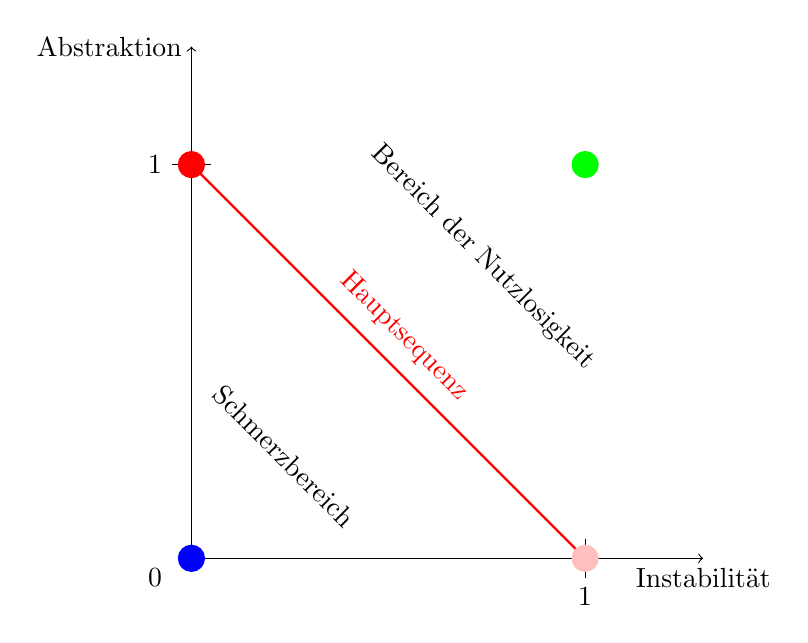
\begin{tikzpicture}[xscale=5,yscale=5,domain=0:1,samples=50]
    \draw[->] (0,0) -- (1.3,0) node[below] {Instabilität};
    \draw[->] (0,0) -- (0,1.3) node[left] {Abstraktion};
    \draw (0.05,1) --  (-0.05,1) node[left] {$1$}; 
    \draw (1,0.05) --  (1,-0.05) node[below] {$1$}; 
    \draw[red,thick] plot (\x,{1-\x});
    \node[label={[red, rotate=-45] Hauptsequenz}] at (0.5,0.5) {};
    \node[label={[rotate=-45] Schmerzbereich}] at (0.2,0.2) {};
    \node[label={[rotate=-45] Bereich der Nutzlosigkeit}] at (0.7,0.7) {};
    \node[below,left] at (-0.05,-0.05) {0};
    \node[draw,green,shape=circle,fill] at (1,1) {};
    \node[draw,blue,shape=circle,fill] at (0,0) {};
    \node[draw,pink,shape=circle,fill] at (1,0) {};
    \node[draw,red,shape=circle,fill] at (0,1) {};
\end{tikzpicture}
\caption{AI-Graph \cite{Mar94}}
\label{fig:ai-graph}
\end{figure}

\subsection{Beispielanalyse von Sweet Home 3D}

Die Martin-Metriken lassen sich wie in Abb.
\ref{fig:martinAnfrage} abfragen. Wenn die ThirdParty Packages
unterdrückt werden sollten, dann müssen CA und CE durch die
Anweisung unter dem Strich ersetzt werden; dies wird im Folgenden
angenommen. Der Betrag in der Martin wurde hierbei weggelassen,
um identifizieren zu können, ob die Packages sich tendenziell im
Schmerzbereich oder im Bereich der Nutzlosigkeit befindet. Die
Ausgabe ist in Abb.  \ref{fig:martinResultOhneThirdParty} und die
Visualiserung der Martin Metrik mit gleicher Rechteckgröße aller
Packages in Abb.  \ref{fig:martinAnfrage}. Ist das Package grün
bewegt sich das Package im Bereich der Nutzlosigkeit, bei Gelb
zum ausbalancierten Bereich und bei Rot zum Schmerzbereich. Aus
den Darstellungen erkennt man, dass die Packages sich eher im
Bereich zum Schmerzbereich bewegen. Dies ist auch nicht
verwunderlich, da in der Ausgabe erkennbar ist, dass der
Abstraktionsgrad bei allen Package relativ niedrig ist.
Insbesonders fällt das Package com.eteks.sweethome3d.tools mit
einem Wert von -0.89 und in der Visualisierung durch eine
dunkel-rote Färbung auf. Hier müsste dann untersucht werden,
inwiefern ein Aufbau des Abstraktionsniveaus möglich und sinnvoll
ist. 


\begin{figure} 
  \centering
  \makebox[\textwidth][c]{\includegraphics[width=\textwidth]{../Images/martinAnfrage.PNG}}
  --------------------------
  \makebox[\textwidth][c]{\includegraphics[width=.6\textwidth]{../Images/martinAnfrageOhneThirdParty.PNG}}
  \caption{Anfrage aller Martin Metriken in CQLinQ mit ThirdParty
  und unter dem Strich Ergänzung ohne ThirdParty}
  \label{fig:martinAnfrage}
\end{figure}

\begin{figure} 
  \centering
  \makebox[\textwidth][c]{\includegraphics[width=\textwidth]{../Images/martinResultOhneThirdParty.PNG}}
  \caption{Ausgabe der Anfrage in Abb. \ref{fig:martinAnfrage}
  ohne ThirdParty}
  \label{fig:martinResultOhneThirdParty}
\end{figure}

\begin{figure} 
  \centering
  \makebox[\textwidth][c]{\includegraphics[width=\textwidth]{../Images/martinOhneThirdParty.png}}
  \caption{Tree Map der Martin Metrik ohne ThirdParty aus Abb.
          \ref{fig:martinResultOhneThirdParty}}
  \label{fig:martin}
\end{figure}

\section{PMD}\label{tools}

JArchitect ist ein kommerzielles Analysewerkzeug und kann aus
urheberrechtlichen Gründen nicht für dritte Programm genutzt
werden. Aus diesem Grund wird das Open-Source Tool PMD
vorgestellt. PMD ist ein plattformunabhängiges Analysewerkezeug
und untersucht neben Java-Code , wie JArchitect, auch
Programmiersprachen wie JavaScript, PLSQL, Apache Velocity usw.
Es bietet z.B. die Möglichkeit Programmwarnungen für ungenutzte
Variabeln, leere Catch-Blöcke etc. auszugeben. Zudem wurde in PMD
ein CPD integriert, dass im Code nach Redundanz sucht und
ausgibt.\\
\\
Im Gegensatz zu den Regel bei JArchitect, basieren die
Regeln häufig nicht auf Metriken, sondern
\\
\\
Die meisten Regel



\section{Fazit}\label{fazit}

\newpage

\bibliographystyle{alphadin}
\bibliography{../Literatur/lit}{}

\end{document}
